\section{Configuração Servidores}

\subsection{Servidor DNS}

Para realizar a resolução de nomes da infraestrutura da empresa, foi implantado um servidor DNS utilizando o software BIND9 na rede do Data Center (DC). O servidor foi configurado como autoridade para o domínio interno \texttt{conectanet.local}, permitindo que os dispositivos da rede acessem os serviços internos por meio de nomes em vez de endereços IP.

A configuração da zona direta foi realizada no arquivo \texttt{/etc/bind/db.conectanet.local}, onde foram cadastrados os registros do tipo \textit{A} para os principais serviços da infraestrutura. Dessa forma, os nomes \texttt{web.conectanet.local}, \texttt{sftp.conectanet.local} e \texttt{dns.conectanet.local} passaram a ser resolvidos para seus respectivos endereços IP, conforme apresentado na Tabela~\ref{tab:dns}.

\begin{table}[H]
\centering
\caption{Registros DNS da zona \texttt{conectanet.local}.}
\label{tab:dns}
\begin{tabular}{ll}
\hline
\textbf{Nome} & \textbf{Endereço IP} \\ \hline
dns.conectanet.local & 172.24.30.12 \\
web.conectanet.local & 172.24.10.14 \\
sftp.conectanet.local & 172.24.10.15 \\ \hline
\end{tabular}
\end{table}

Além da resolução de nomes internos, o servidor DNS foi configurado para encaminhar consultas referentes a domínios externos para o servidor DNS institucional da Universidade de Brasília (UnB), localizado no endereço \texttt{172.16.4.2}. Essa configuração foi realizada por meio do mecanismo de \textit{forwarders} do BIND, permitindo que consultas a domínios públicos, como \texttt{google.com}, fossem resolvidas corretamente sem a necessidade de o servidor realizar consultas diretamente aos servidores raiz da Internet.

Após a configuração, os clientes das redes Intranet, DMZ e Data Center passaram a utilizar o servidor DNS interno para resolução de nomes locais e externos. Dessa forma, tornou-se possível acessar os serviços da infraestrutura utilizando nomes amigáveis, como \texttt{web.conectanet.local} e \texttt{sftp.conectanet.local}, em substituição aos respectivos endereços IP.

\subsection{Servidor Web (Nginx)}

O servidor Web foi implementado utilizando o \textit{Nginx}, instalado em uma máquina Linux denominada \textit{Web}, localizada na rede DMZ. O servidor possui endereço IP \textit{172.24.10.14} e tem como finalidade disponibilizar páginas Web por meio do protocolo HTTP.

Após a instalação do serviço, foi criada uma página personalizada para validar o funcionamento do servidor e demonstrar sua publicação na rede DMZ. O acesso ao servidor é realizado a partir das máquinas autorizadas conforme as regras configuradas no firewall, permitindo apenas o tráfego destinado ao serviço Web.

\subsection{Servidor SFTP}

O servidor SFTP foi configurado na máquina \textit{SFTP}, localizada na rede DMZ, utilizando o serviço OpenSSH. Inicialmente foi realizada a instalação do servidor SSH, responsável por fornecer o serviço SFTP por meio da porta TCP 22.

\begin{listing}[H]
\centering
\begin{minted}[
bgcolor=bgcolor,
frame=lines,
breaklines=true,
breakanywhere=true,
fontsize=\footnotesize]{bash}
sudo apt update
sudo apt install openssh-server -y
\end{minted}
\caption{Instalação do serviço OpenSSH.}
\label{lst:installSSH}
\end{listing}

Após a instalação, o serviço foi habilitado para iniciar automaticamente durante a inicialização do sistema operacional.

\begin{listing}[H]
\centering
\begin{minted}[
bgcolor=bgcolor,
frame=lines,
breaklines=true,
breakanywhere=true,
fontsize=\footnotesize]{bash}
sudo systemctl enable ssh
sudo systemctl start ssh
\end{minted}
\caption{Inicialização do serviço SSH.}
\label{lst:startSSH}
\end{listing}

Após a configuração, o serviço foi reiniciado para aplicar as alterações.

\begin{listing}[H]
\centering
\begin{minted}[
bgcolor=bgcolor,
frame=lines,
fontsize=\footnotesize]{bash}
sudo systemctl restart ssh
\end{minted}
\caption{Reinicialização do serviço SSH.}
\label{lst:restartSSH}
\end{listing}

O acesso ao servidor é realizado utilizando o comando:

\begin{center}
\texttt{sftp user@172.24.10.15}
\end{center}



\subsection{Configuração do Servidor Samba}

Com o objetivo de disponibilizar um serviço de compartilhamento de arquivos na rede corporativa, foi implantado um servidor Samba na rede do Data Center (DC). O Samba foi escolhido por implementar o protocolo SMB/CIFS, amplamente utilizado para compartilhamento de arquivos e impressoras entre sistemas Linux e Windows.

Inicialmente, foi realizada a instalação do pacote \texttt{samba} no servidor Linux, seguida da configuração do arquivo \texttt{/etc/samba/smb.conf}. Nesse arquivo foram definidos os parâmetros globais do servidor, como o grupo de trabalho (\textit{workgroup}), o nome do servidor e as configurações de autenticação dos usuários.

Em seguida, foi criado um diretório destinado ao compartilhamento de arquivos, com as permissões adequadas para acesso pelos usuários autorizados. O compartilhamento foi configurado para permitir autenticação por usuário, garantindo que somente usuários previamente cadastrados no sistema e no banco de usuários do Samba pudessem acessar os arquivos disponibilizados.

Após a criação dos usuários no sistema operacional, foi utilizado o comando \texttt{smbpasswd} para cadastrá-los no banco de autenticação do Samba, permitindo o acesso ao compartilhamento por meio de credenciais individuais.

Para validar a configuração, foram realizados testes de acesso a partir de máquinas clientes da rede, utilizando tanto o endereço IP quanto o nome do servidor resolvido pelo serviço DNS interno. Os clientes conseguiram estabelecer conexão com o compartilhamento, realizar operações de leitura, gravação e exclusão de arquivos conforme as permissões configuradas, comprovando o correto funcionamento do serviço.

A utilização do servidor Samba centraliza o armazenamento dos arquivos compartilhados da organização, facilita o gerenciamento de permissões de acesso e proporciona interoperabilidade entre diferentes sistemas operacionais presentes na infraestrutura da rede.

\subsection{Servidor Zabbix}

Inicialmente, foi realizada a instalação do servidor Zabbix seguindo os procedimentos descritos na documentação oficial. Durante a configuração, foram realizadas alterações no arquivo \texttt{/etc/zabbix/zabbix\_server.conf}, conforme apresentado no Código \ref{lst:ServidoresZabbixServerConf}.

\begin{listing}[H]
\centering
\begin{minted}[
    bgcolor=bgcolor,
    frame=lines,
    breaklines=true,
    breakanywhere=true,
    fontsize=\footnotesize,
]{yaml}

DBName=zabbix
DBUser=zabbix
DBPassword=zabbix

\end{minted}
\caption{Configuração do arquivo zabbix\_server.conf}
\label{lst:ServidoresZabbixServerConf}
\end{listing}

Por fim, os serviços do servidor Zabbix, Nginx e banco de dados foram reiniciados para aplicação das configurações realizadas, conforme mostrado no Código \ref{lst:ServidoresZabbixRestart}.

\begin{listing}[H]
\centering
\begin{minted}[
    bgcolor=bgcolor,
    frame=lines,
    breaklines=true,
    breakanywhere=true,
    fontsize=\footnotesize,
]{bash}

sudo systemctl restart zabbix-server
sudo systemctl restart nginx
sudo systemctl restart postgresql

\end{minted}
\caption{Reinicialização dos serviços do servidor Zabbix}
\label{lst:ServidoresZabbixRestart}
\end{listing}

Após o acesso ao Zabbix web, foi necessária a configuração de todos os dispositivos. Para isso, foram acessadas as abas \textit{Monitoring->Hosts} e adicionados todos os hosts pelos passos da Figura \ref{fig:zabbix}. O primeiro passo para essa configuração foi: (a) nome do host; (b) template SNMP utilizado; (c) grupo do host; (d) interface SNMP configurada.

\begin{figure}[H]
    \centering
    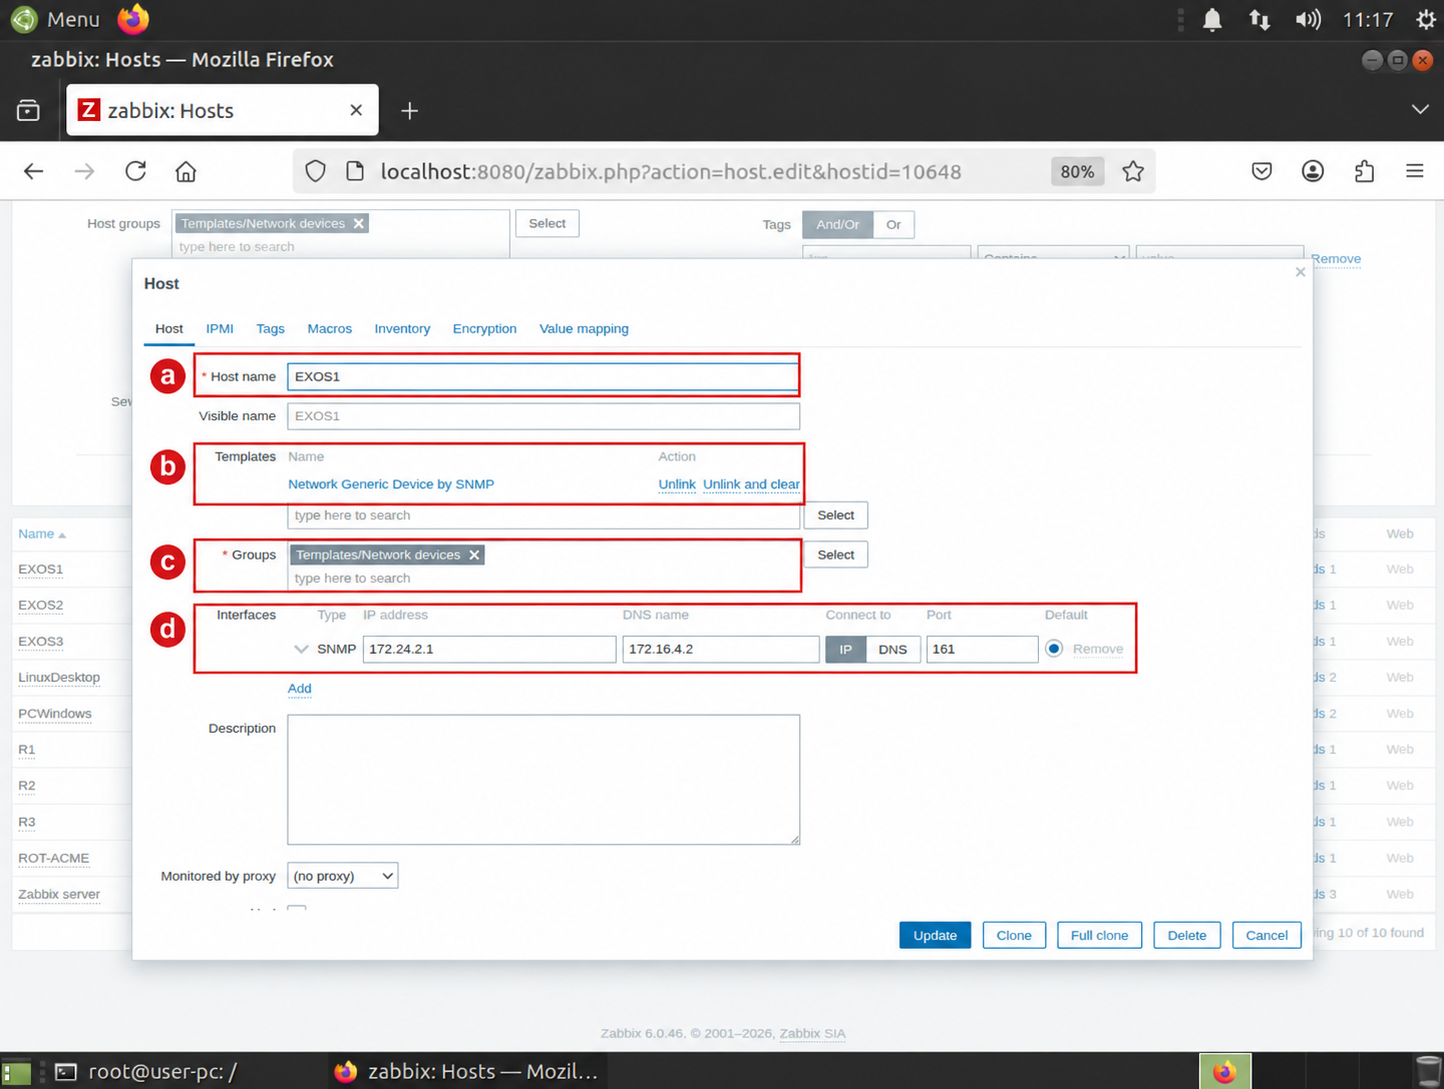
\includegraphics[width=1\linewidth]{zabbix.png}
    \caption{Configuração do host EXOS1 no Zabbix: (a) nome do host; (b) template SNMP utilizado; (c) grupo do host; (d) interface SNMP configurada.}
    \label{fig:zabbix}
\end{figure}

\subsection{Grafana}

Inicialmente, foi necessário acessar o menu de administração do Grafana para realizar a instalação e configuração dos plug-ins utilizados no monitoramento da infraestrutura. Conforme apresentado na Figura~\ref{fig:grafanaAdm}, acessa-se o menu \textit{Administração}, em seguida a opção \textit{Plug-ins e dados} e, posteriormente, \textit{Plug-ins}.

\begin{figure}[H]
    \centering
    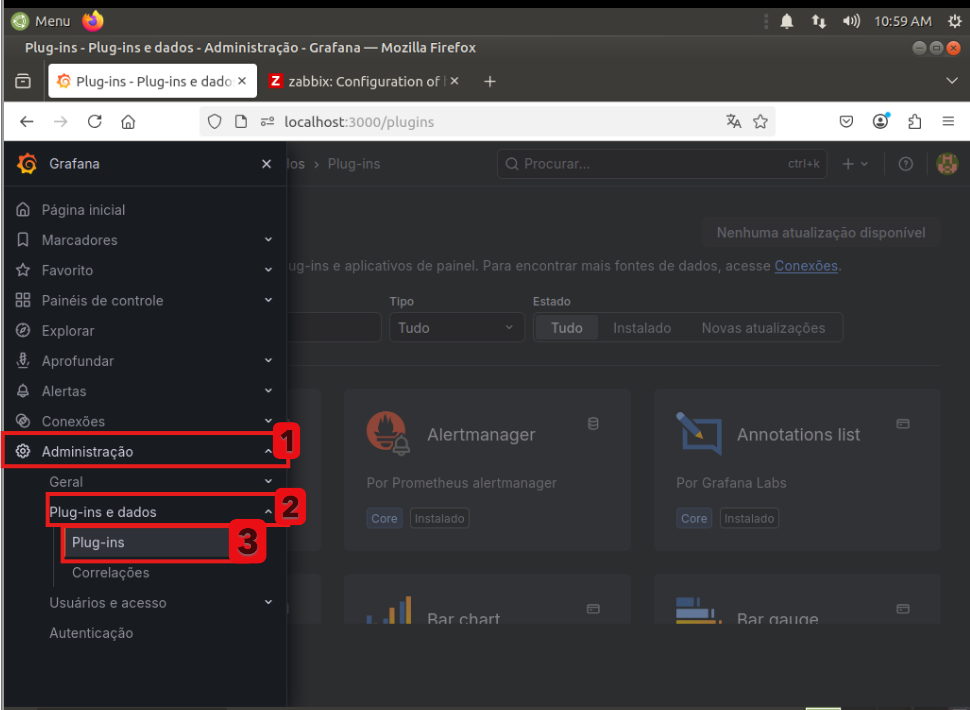
\includegraphics[width=1\linewidth]{fig/zabbix/grafanaAdm.png}
    \caption{Acesso ao menu de gerenciamento de plug-ins do Grafana: 1. Administração; 2. Plug-ins e dados; 3. Plug-ins.}
    \label{fig:grafanaAdm}
\end{figure}

Após acessar a área de plug-ins, realizou-se a pesquisa do plug-in PostgreSQL utilizando o campo de busca. Em seguida, selecionou-se o plug-in correspondente, conforme ilustrado na Figura~\ref{fig:grafanaPostgreP}.

\begin{figure}[H]
    \centering
    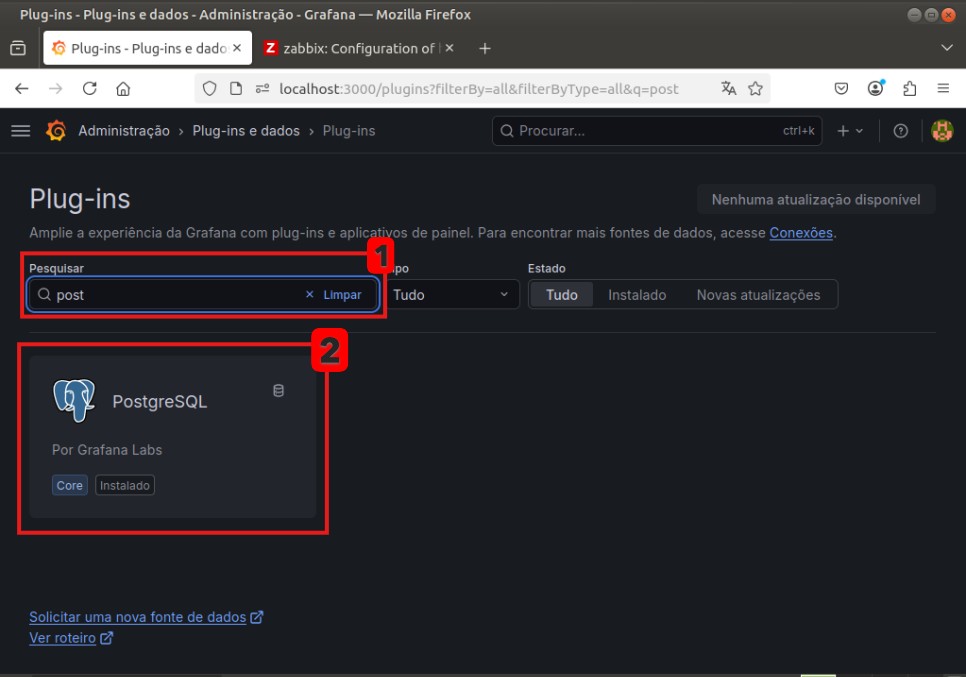
\includegraphics[width=1\linewidth]{fig/zabbix/grafanaPostgreP.png}
    \caption{Pesquisa do plug-in PostgreSQL: 1. Campo de pesquisa; 2. Plug-in PostgreSQL.}
    \label{fig:grafanaPostgreP}
\end{figure}

A Figura~\ref{fig:grafanaPostgresE} apresenta a página do plug-in PostgreSQL no Grafana, utilizada para confirmar a instalação e possibilitar a adição de uma nova fonte de dados baseada em PostgreSQL.

\begin{figure}[H]
    \centering
    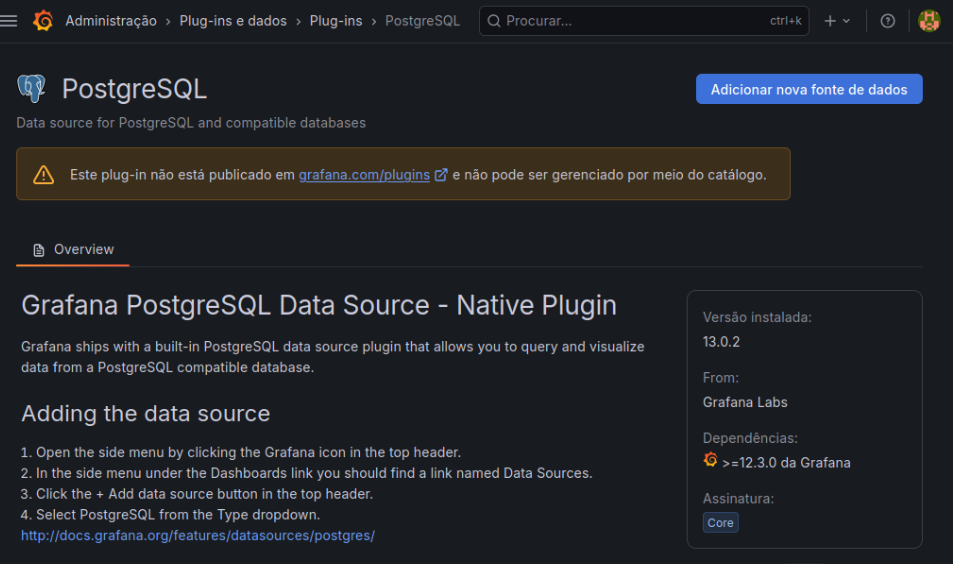
\includegraphics[width=1\linewidth]{fig/zabbix/grafanaPostgresE.png}
    \caption{Página do plug-in PostgreSQL no Grafana.}
    \label{fig:grafanaPostgresE}
\end{figure}

De maneira semelhante, realizou-se a pesquisa do plug-in Zabbix no catálogo de plug-ins do Grafana. Conforme mostrado na Figura~\ref{fig:grafanaZabbixP}, foi utilizado o campo de pesquisa para localizar o plug-in Zabbix e selecioná-lo para configuração.

\begin{figure}[H]
    \centering
    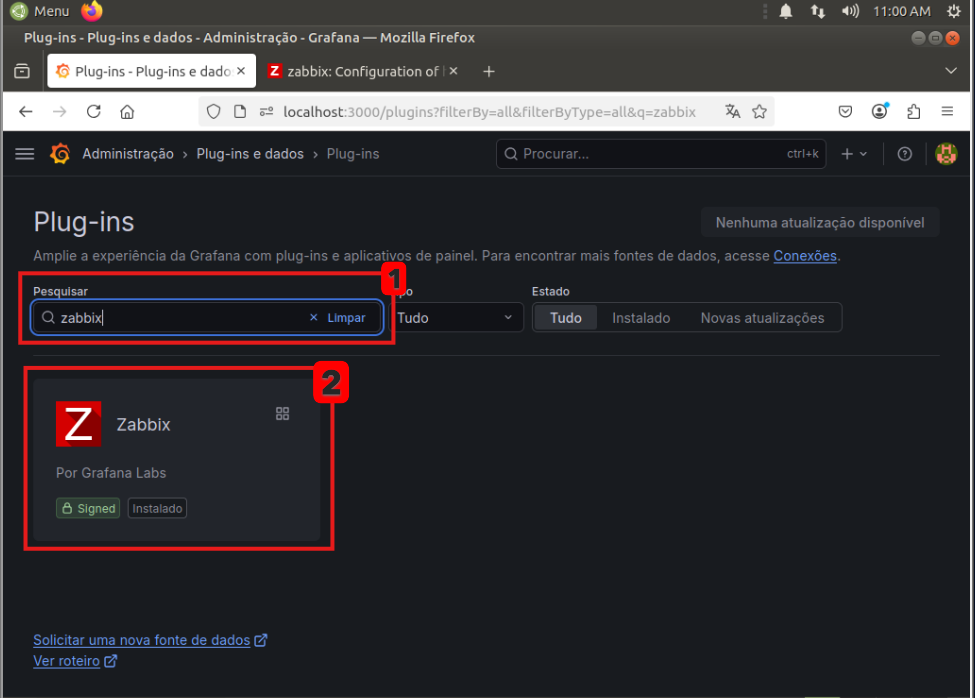
\includegraphics[width=1\linewidth]{fig/zabbix/grafanaZabbixP.png}
    \caption{Pesquisa do plug-in Zabbix: 1. Campo de pesquisa; 2. Plug-in Zabbix.}
    \label{fig:grafanaZabbixP}
\end{figure}

Por fim, a Figura~\ref{fig:grafanaZabbixE} apresenta a tela do plug-in Zabbix já instalado no Grafana, permitindo sua ativação e integração com o sistema de monitoramento.

\begin{figure}[H]
    \centering
    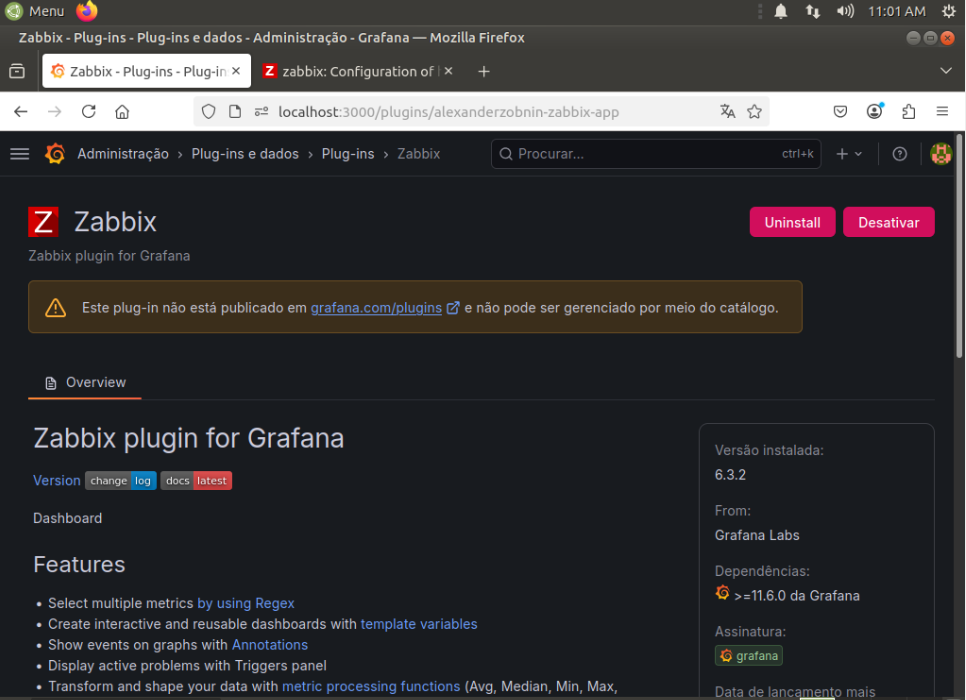
\includegraphics[width=1\linewidth]{fig/zabbix/grafanaZabbixE.png}
    \caption{Página do plug-in Zabbix no Grafana.}
    \label{fig:grafanaZabbixE}
\end{figure}

Após a instalação dos plug-ins necessários, realizou-se a configuração da conexão entre o Grafana e o Zabbix. Inicialmente, acessou-se o menu de conexões do Grafana e selecionou-se a opção para adicionar uma nova conexão, conforme apresentado na Figura~\ref{fig:conexaoGrafana}.

\begin{figure}[H]
    \centering
    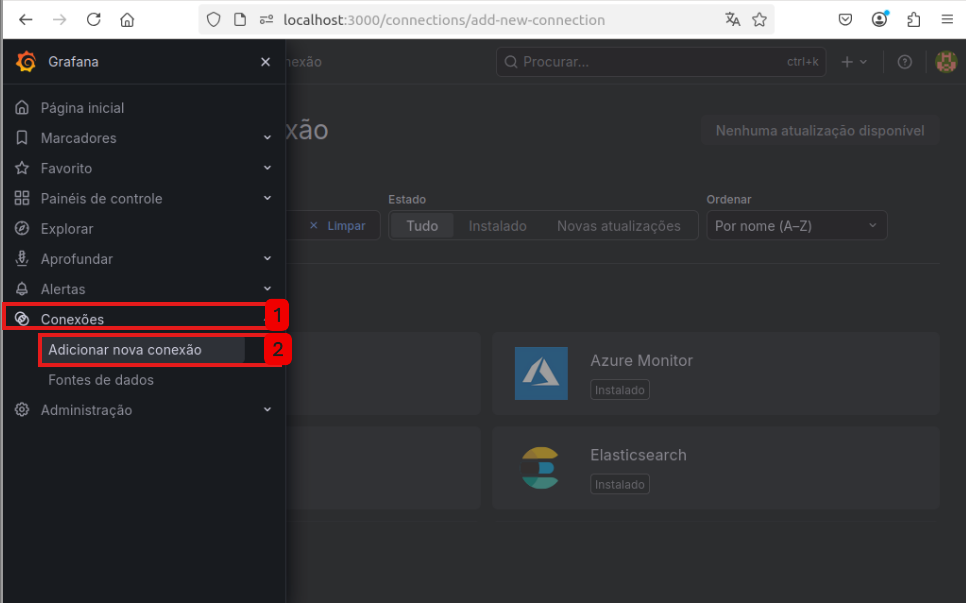
\includegraphics[width=1\linewidth]{fig/zabbix/conexao.png}
    \caption{Acesso ao menu de conexões do Grafana: 1. Conexões; 2. Adicionar nova conexão.}
    \label{fig:conexaoGrafana}
\end{figure}

Em seguida, foi realizada a pesquisa do plug-in Zabbix no catálogo de conexões disponíveis do Grafana. Conforme ilustrado na Figura~\ref{fig:conexaoZabbixPesquisa}, utilizou-se o campo de pesquisa para localizar o Zabbix e selecioná-lo para iniciar a configuração.

\begin{figure}[H]
    \centering
    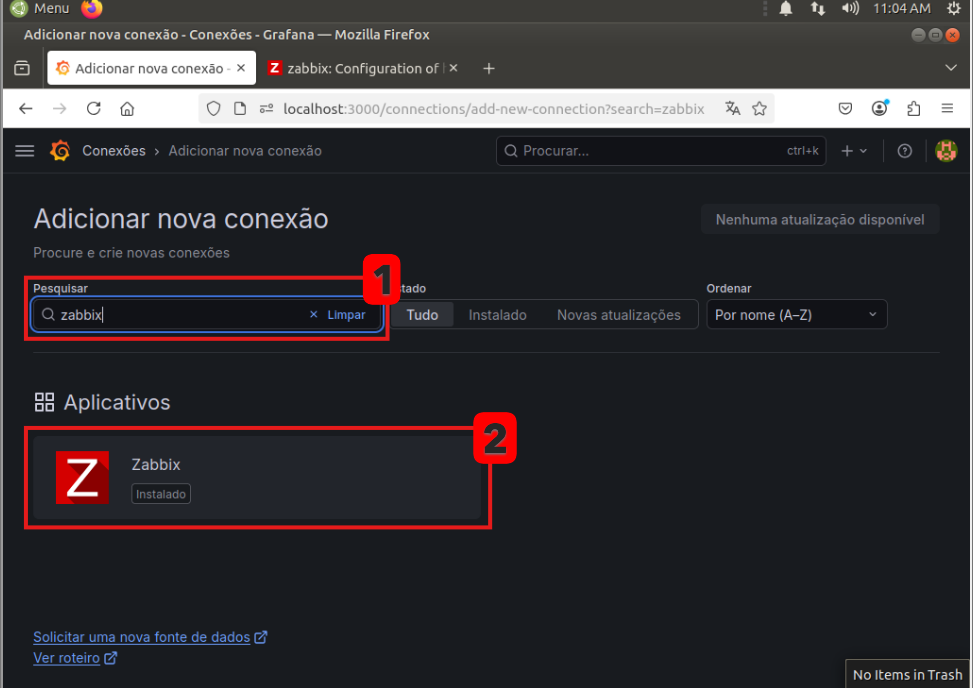
\includegraphics[width=1\linewidth]{fig/zabbix/conexaoZabbix.png}
    \caption{Pesquisa da conexão Zabbix: 1. Campo de pesquisa; 2. Aplicação Zabbix.}
    \label{fig:conexaoZabbixPesquisa}
\end{figure}

Posteriormente, foram configurados os parâmetros iniciais da conexão, incluindo o nome da fonte de dados e a URL da API do Zabbix, conforme mostrado na Figura~\ref{fig:conexaoZabbixConfig}.

\begin{figure}[H]
    \centering
    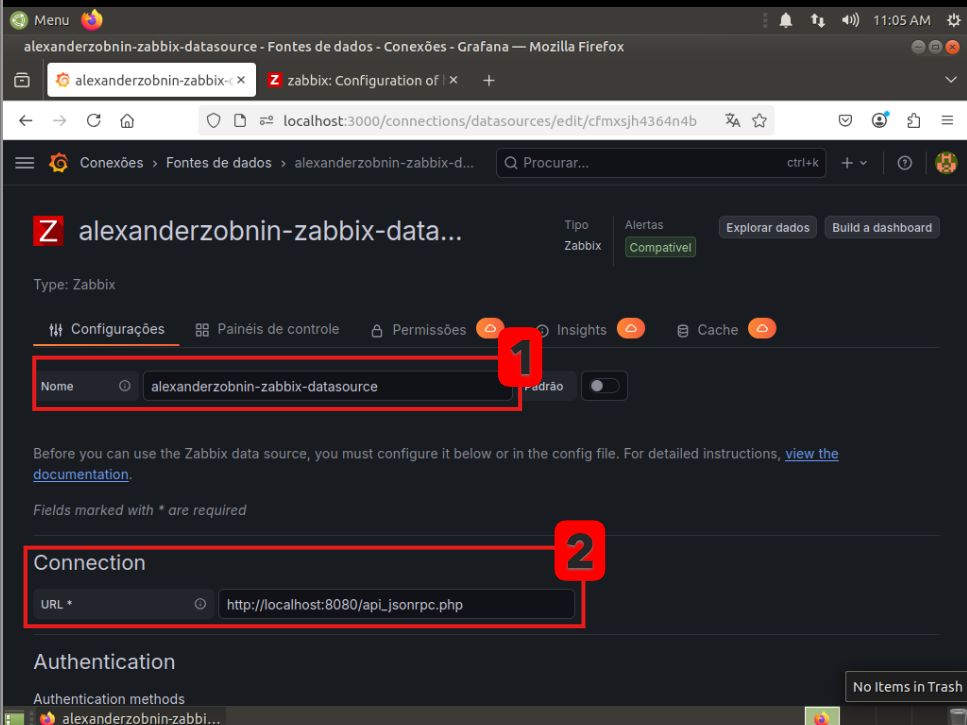
\includegraphics[width=1\linewidth]{fig/zabbix/conexaoZabbix2.png}
    \caption{Configuração inicial da conexão Zabbix: 1. Nome da conexão; 2. URL da API do Zabbix.}
    \label{fig:conexaoZabbixConfig}
\end{figure}

Na sequência, foram definidos os parâmetros de autenticação da conexão, utilizando o método \textit{User and password}, juntamente com as credenciais de acesso ao servidor Zabbix, conforme apresentado na Figura~\ref{fig:conexaoZabbixAuth}.

\begin{figure}[H]
    \centering
    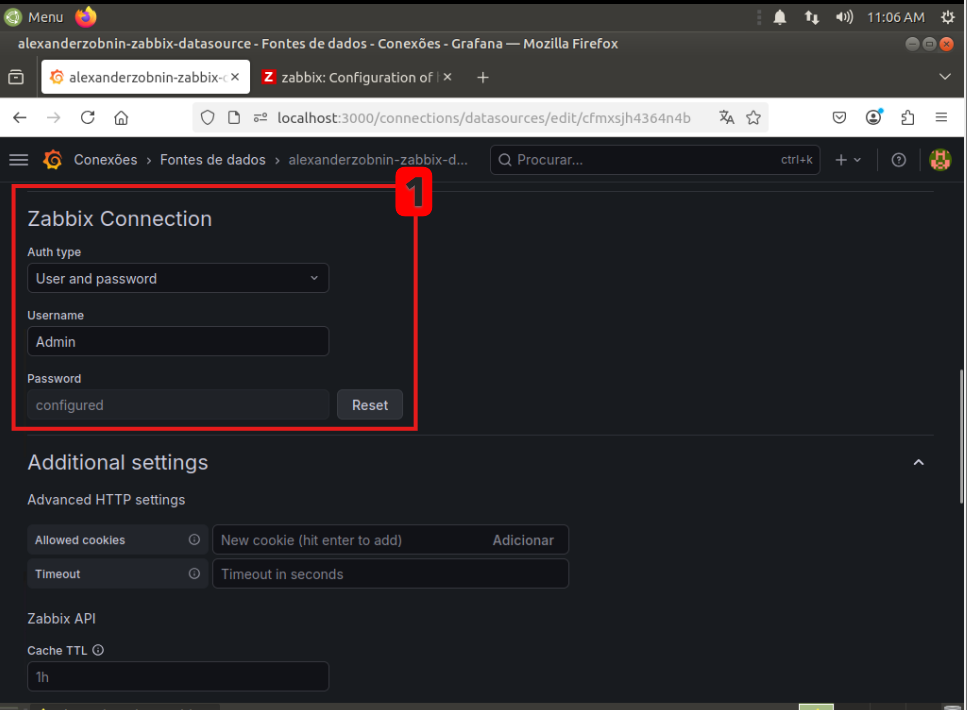
\includegraphics[width=1\linewidth]{fig/zabbix/conexaoZabbix3.png}
    \caption{Configuração de autenticação da conexão Zabbix: 1. Configuração de autenticação e credenciais de acesso.}
    \label{fig:conexaoZabbixAuth}
\end{figure}

Por fim, habilitou-se a opção de conexão direta com o banco de dados PostgreSQL e selecionou-se a fonte de dados correspondente. Após a configuração, utilizou-se a opção \textit{Salvar e testar} para validar a conexão, conforme ilustrado na Figura~\ref{fig:conexaoZabbixFinal}.

\begin{figure}[H]
    \centering
    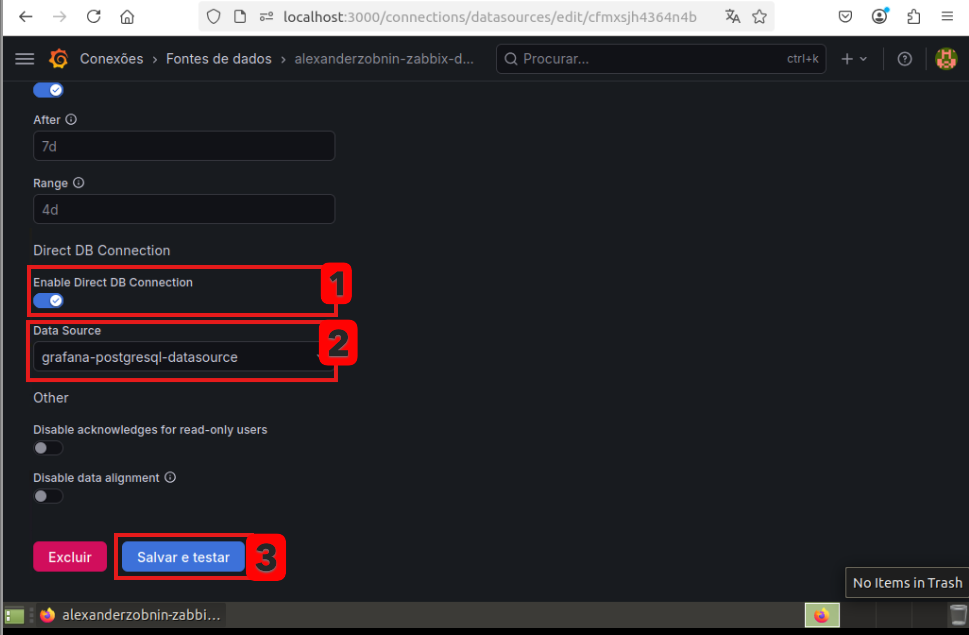
\includegraphics[width=1\linewidth]{fig/zabbix/conexaoZabbix4.png}
    \caption{Configuração final da conexão Zabbix: 1. Habilitar conexão direta; 2. Seleção da fonte de dados PostgreSQL; 3. Salvar e testar conexão.}
    \label{fig:conexaoZabbixFinal}
\end{figure}

\subsection{Criação de painéis no Grafana}

Após a configuração das conexões entre o Grafana, o PostgreSQL e o Zabbix, realizou-se a criação dos painéis de monitoramento utilizados para visualização das métricas da infraestrutura de rede. Inicialmente, acessou-se o menu \textit{Painéis de controle}, conforme apresentado na Figura~\ref{fig:grafanaDashboard1}.

\begin{figure}[H]
    \centering
    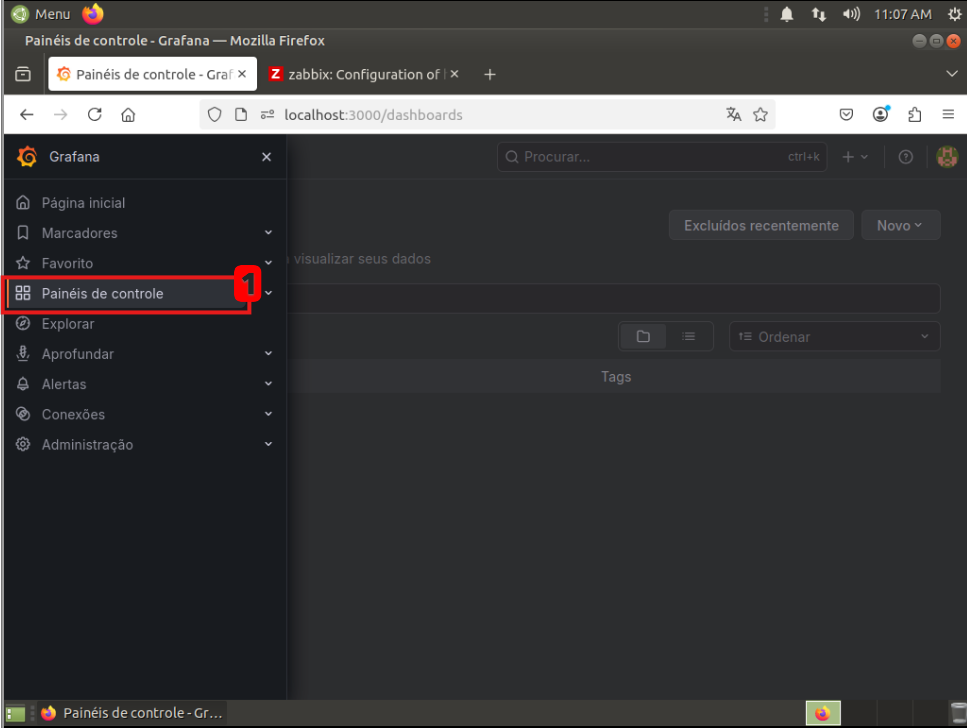
\includegraphics[width=1\linewidth]{fig/zabbix/dashboard1.png}
    \caption{Acesso ao menu de painéis de controle do Grafana: 1. Painéis de controle.}
    \label{fig:grafanaDashboard1}
\end{figure}

Em seguida, foi criado um novo painel por meio da opção \textit{Novo} e, posteriormente, selecionando \textit{Novo painel de controle}, conforme ilustrado na Figura~\ref{fig:grafanaDashboard2}.

\begin{figure}[H]
    \centering
    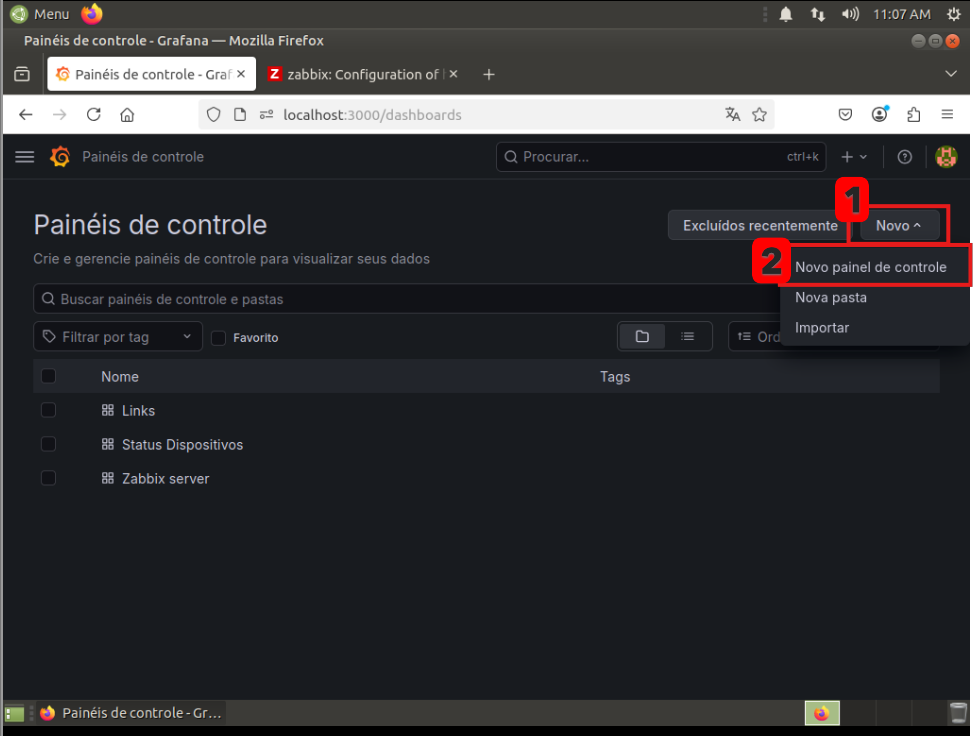
\includegraphics[width=1\linewidth]{fig/zabbix/dashboard2.png}
    \caption{Criação de um novo painel de controle: 1. Menu Novo; 2. Novo painel de controle.}
    \label{fig:grafanaDashboard2}
\end{figure}

Após a criação do painel, adicionou-se uma nova visualização utilizando a opção destacada na Figura~\ref{fig:grafanaDashboard3}.

\begin{figure}[H]
    \centering
    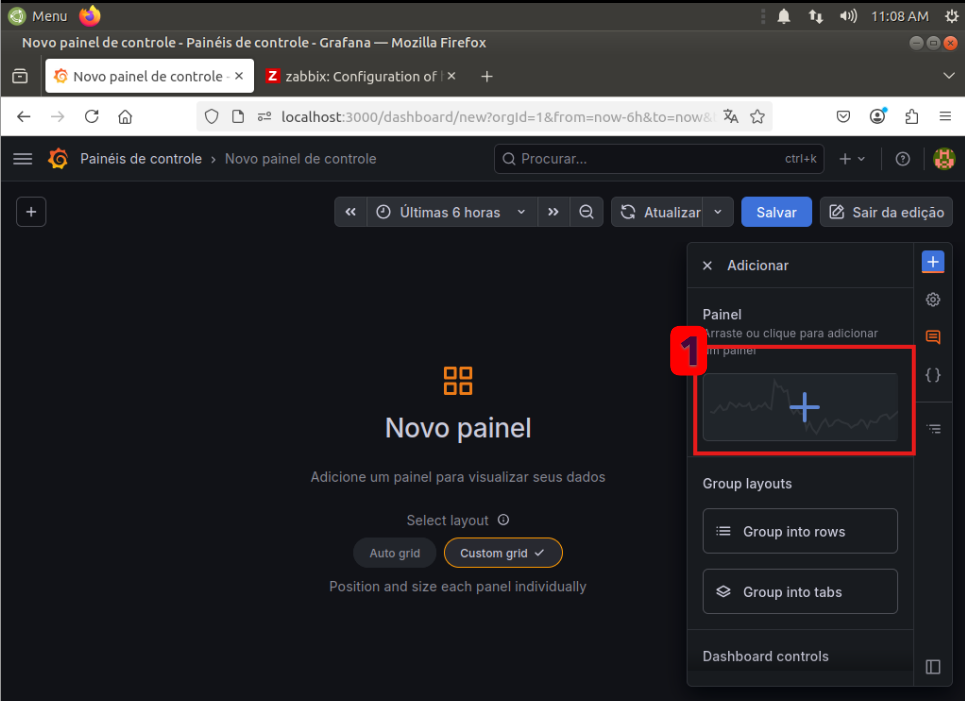
\includegraphics[width=1\linewidth]{fig/zabbix/dashboard3.png}
    \caption{Adição de uma nova visualização ao painel: 1. Adicionar painel.}
    \label{fig:grafanaDashboard3}
\end{figure}

Posteriormente, selecionou-se a opção \textit{Configure visualization} para iniciar a configuração da visualização do painel, conforme mostrado na Figura~\ref{fig:grafanaDashboard4}.

\begin{figure}[H]
    \centering
    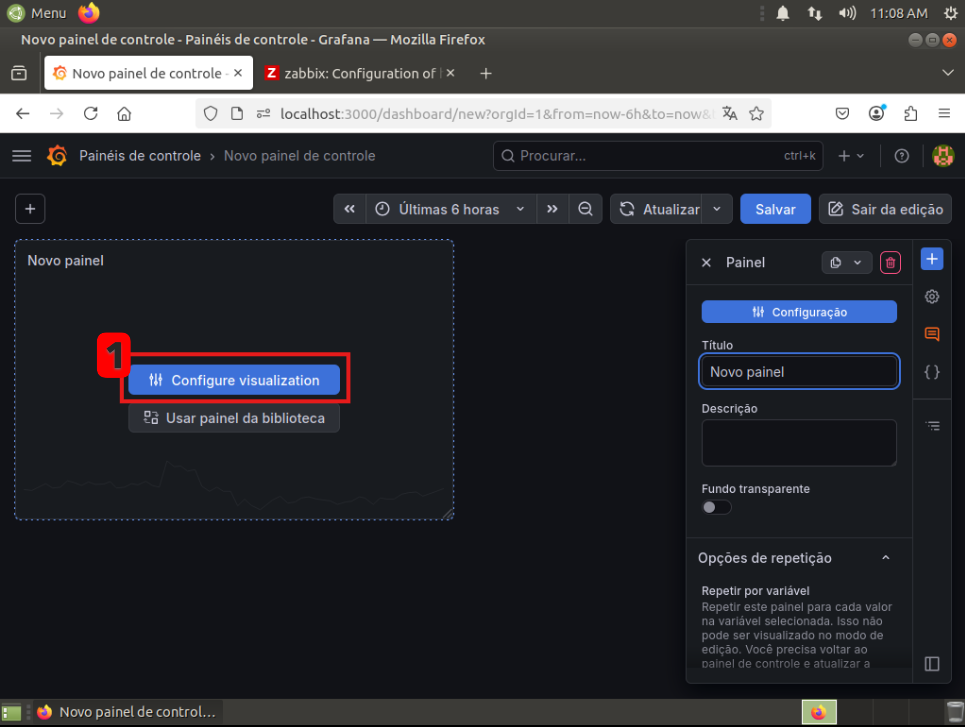
\includegraphics[width=1\linewidth]{fig/zabbix/dashboard4.png}
    \caption{Configuração da visualização do painel: 1. Configure visualization.}
    \label{fig:grafanaDashboard4}
\end{figure}

Na etapa seguinte, foi realizada a configuração da consulta utilizada para exibição das métricas do Zabbix. Conforme apresentado na Figura~\ref{fig:grafanaDashboard5}, definiu-se a fonte de dados, o tipo de consulta, o grupo, o host, a tag do item, o item monitorado e a visualização do painel.

\begin{figure}[H]
    \centering
    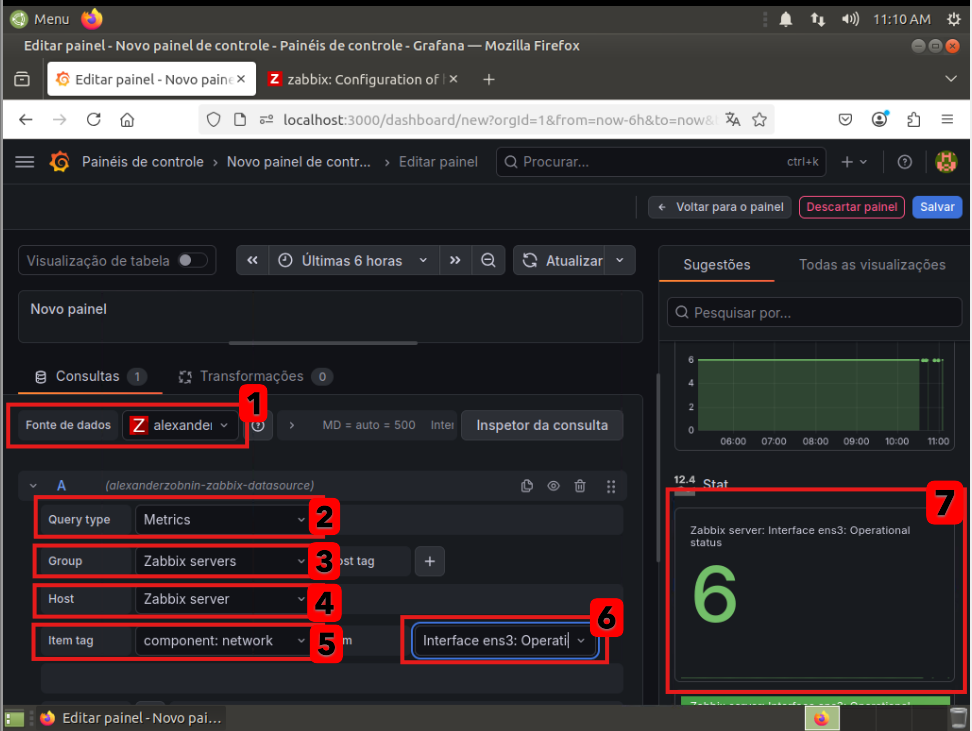
\includegraphics[width=1\linewidth]{fig/zabbix/dashboard5.png}
    \caption{Configuração da consulta do painel: 1. Fonte de dados; 2. Tipo de consulta; 3. Grupo; 4. Host; 5. Tag do item; 6. Item monitorado; 7. Visualização do painel.}
    \label{fig:grafanaDashboard5}
\end{figure}

Por fim, após a configuração do painel, utilizou-se a opção \textit{Salvar} para armazenar o dashboard criado no Grafana, conforme ilustrado na Figura~\ref{fig:grafanaDashboard6}.

\begin{figure}[H]
    \centering
    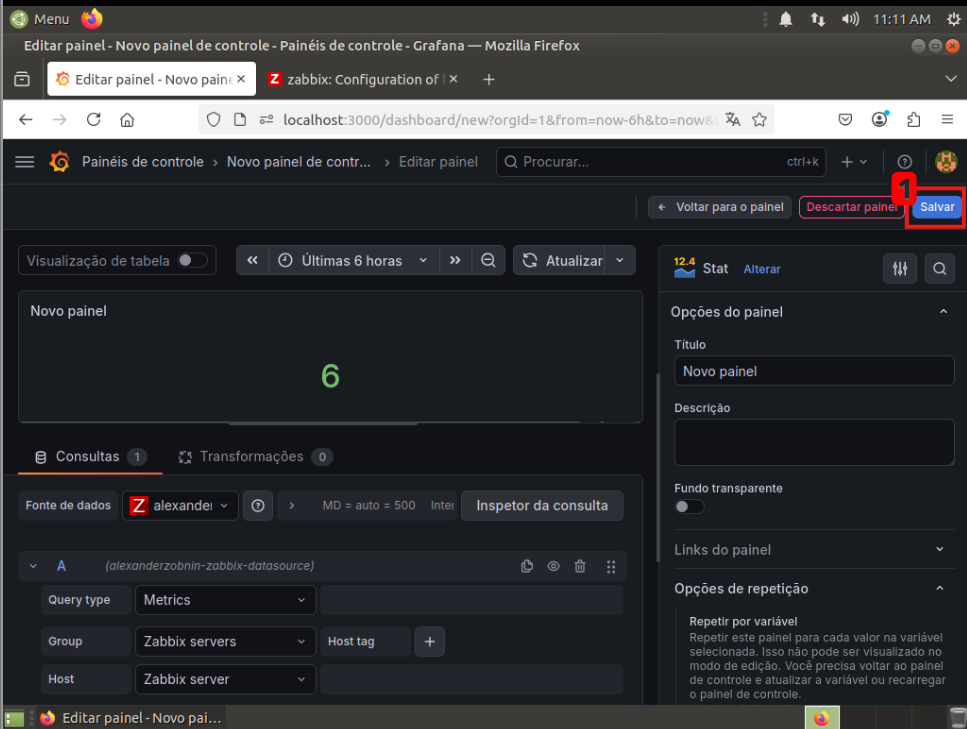
\includegraphics[width=1\linewidth]{fig/zabbix/dashboard6.png}
    \caption{Salvamento do painel configurado: 1. Botão Salvar.}
    \label{fig:grafanaDashboard6}
\end{figure}
